\documentclass[11pt]{exam}
\RequirePackage{amssymb, amsfonts, amsmath, latexsym, verbatim, xspace, setspace}
\RequirePackage{tikz, pgflibraryplotmarks}

\usepackage[margin=1in]{geometry}
\usepackage[utf8]{inputenc}


% Here's where you edit the Class, Exam, Date, etc.
\newcommand{\class}{Seminario de tecnología}
\newcommand{\examnum}{Examen Parcial 3}
\newcommand{\term}{2 Cuatrimestre, 2014}
\newcommand{\examdate}{14/11/14}
\newcommand{\timelimit}{120 minutos}

% For an exam, single spacing is most appropriate
\singlespacing
% \onehalfspacing
% \doublespacing

% For an exam, we generally want to turn off paragraph indentation
\parindent 0ex

\begin{document} 

% These commands set up the running header on the top of the exam pages
\pagestyle{head}
\firstpageheader{}{}{}
\runningheader{\class}{\examnum\ - Pagina \thepage\ de \numpages}{\examdate}
\runningheadrule

\begin{flushright}
\begin{tabular}{p{2.8in} r l}
\textbf{\class} & \textbf{Nombre:} & \makebox[2in]{\hrulefill}\\
\textbf{\term} &&\\
\textbf{\examnum} &&\\
\textbf{\examdate} &&\\
\textbf{Tiempo: \timelimit}
\end{tabular}\\
\end{flushright}
\rule[1ex]{\textwidth}{.1pt}

\begin{minipage}[t]{3.7in}
Este examen consta de \numpages\ paginas y \numquestions\ preguntas. Verifique que tiene todas las hojas necesarias. Las preguntas se responden en la misma hoja del examen.\\

El examen se puede realizar a libro abierto y esta permitido el uso de calculadora si es requerido. Se puede utilizar computadora.\\

Las siguientes reglas aplican para la aprobación del examen:\\
\vspace{0pt}
\begin{itemize}
\item Escritura de todas las \textbf{respuestas en tinta, sin excepción}.-
\item \textbf{Se requiere un mínimo de 4 puntos} para la aprobación del examen.-
\item Justificar sus respuestas, en caso de ser necesario, con diagramas o ejemplos claro.-
\item Lea todo el examen antes de comenzar a responder. Algunas preguntas guardan relación con otras y pueden servir de ayuda.-
\end{itemize}

No escriba en la tabla de la derecha.\\
\\
\textbf{Mucha suerte! :)}

\end{minipage}
\hfill
\begin{minipage}[t]{2.3in}
\vspace{0pt}
%\cellwidth{3em}
\gradetablestretch{2}
\vqword{Pregunta}
\addpoints % required here by exam.cls, even though questions haven't started yet.	
\gradetable[v]%[pages]  % Use [pages] to have grading table by page instead of question

\end{minipage}
\newpage % End of cover page

%%%%%%%%%%%%%%%%%%%%%%%%%%%%%%%%%%%%%%%%%%%%%%%%%%%%%%%%%%%%%%%%%%%%%%%%%%%%%%%%%%%%%
%
% See http://www-math.mit.edu/~psh/#ExamCls for full documentation, but the questions
% below give an idea of how to write questions [with parts] and have the points
% tracked automatically on the cover page.
%
%
%%%%%%%%%%%%%%%%%%%%%%%%%%%%%%%%%%%%%%%%%%%%%%%%%%%%%%%%%%%%%%%%%%%%%%%%%%%%%%%%%%%%%

\begin{questions}

% Pregunta 1
\addpoints
\question[2] Defina el concepto de Minería de datos.
\vspace{2in}

% Pregunta 2
\addpoints
\question[1] Indique cual/es de las siguientes herramientas se utilizan para análisis estadístico de clusters:
\begin{itemize}
\item SPSS
\item Weka
\item Qucs
\end{itemize}

% Pregunta 3
\addpoints
\question[2] Describa las etapas del proceso de generación de un modelo de minería de datos.
%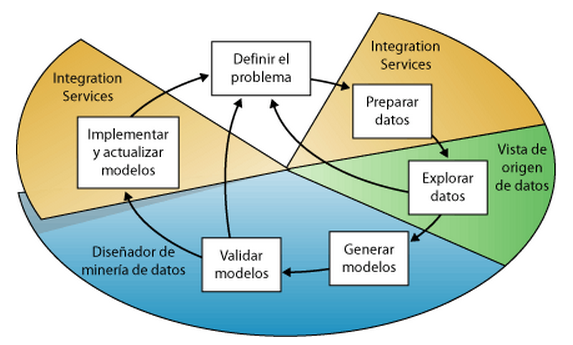
\includegraphics[scale=0.35]{steps}
\vspace{2in}


% Pregunta 4
\addpoints
\question[1] \textbf{Indique la opcion correcta.} El modelo de minería de datos que crea un algoritmo a partir de los datos puede tomar diversas formas, incluyendo:

\begin{enumerate}
\item Un conjunto de clústeres que describe cómo se relacionan los casos de un conjunto de datos.
\item Un árbol de decisión que predice un resultado y que describe cómo afectan a este los distintos criterios.
\item Un modelo matemático que predice las ventas.
\item Un conjunto de reglas que describen cómo se agrupan los productos en una transacción, y las probabilidades de que dichos productos se adquieran juntos.
\item Ninguno de los anteriores
\item Los itemas 1, 2, 3 y 4.
\end{enumerate}


\newpage
% Pregunta 5
\addpoints
\question[1] Los algoritmos para el análisis de datos se pueden elegir, entre otros cosas, según el tipo de análisis que se quiere realizar. Mencione brevemente esta clasificación.
\vspace{2in}

% Pregunta 6
\addpoints
\question[1] \textbf{Indique la opción correcta.} La configuración de una estructura de minería de datos consta de 5 pasos. Marque cual de ellos \textit{\textbf{es opcional}}.

\begin{itemize}
\item Definir un origen de datos.
\item Seleccionar las columnas de datos que se van a incluir en la estructura (no es necesario agregar todas las columnas al modelo) y definir una clave.
\item Definir una clave para la estructura, incluyendo la clave de la tabla anidada, si procede.
\item Especificar si los datos de origen se deben separar en un conjunto de entrenamiento y en un conjunto de prueba.
\item Procesar la estructura.
\end{itemize}

% Pregunta 7
\addpoints
\question[1] Defina el concepto de outlier.
\vspace{1in}

% Pregunta 8
\addpoints
\question[1] Existen 3 (tres) criterios para validar los modelos de minería de datos. Cuales son?
\vspace{4.5in}
\end{questions}
\end{document}